
\section{Going beyond the SM with vector-like quarks}\label{sec:THvlq}

New physics models proposed to go BSM have been briefly presented in
Section~\ref{sec:THquest}. Some of these theories predict new heavy
quarks~\cite{AguilarSaavedra:2009es} %,Martin:2009bg}
with spin 1/2, transforming as triplets under $SU(3)_C$ and 
%and whose left- and right-handed components have the same colour and electroweak quantum numbers.
 with the same electroweak quantum numbers for their 
left- and right-handed components. They will
therefore transform the same under 
$SU(2)_L\otimes U(1)_Y$. 
This also means that those new quarks will not
contribute to the Higgs production and decay 
processes, avoiding then the
limitations encountered by a fourth chiral generation hypothesis.

In this section is described the general phenomenology of new heavy top and bottom
partners, $T$ and $B$ with charges $2/3$ and $-1/3$ respectively, as
well as new heavy exotic quarks, $X$ and $Y$ with charges $5/3$ and 
$-4/3$ respectively. They can appear, depending on the model considered,
as  $\text{SU}(2)_L$ isosinglets, isodoublets or isotriplets, but here
only the first two cases will be considered. 
A new $T_{L,R}$ isosinglet is present, e.g., in 
Little Higgs models~\cite{ArkaniHamed:2001nc,Perelstein:2005ka}, 
%ArkaniHamed:2002qy,
where it aids solving the hierarchy problem, as well
as (in form of a tower of isosinglets $T_{L,R}^{(n)}$) 
in extra-dimensional models with $t_R$ 
in the bulk~\cite{Csaki:2004ay}. 
%~\cite{Mirabelli:1999ks,Chang:1999nh,Csaki:2004ay}. % of which the lightest one can be light and have sizeable mixing with the third generation~\cite{delAguila:2000kb}. 
%More recently, $\TB_{L,R}$ and $\XT_{L,R}$ isodoublets of hypercharges $1/6$, $7/6$ coupling to the third generation naturally emerge~\cite{Contino:2006qr,Carena:2006bn} in warped models implementing a custodial symmetry to protect the $Zbb$ coupling~\cite{Agashe:2006at}. Charge $-1/3$ isosinglets $B_{L,R}$ are predicted in grand unification theories based on $\Esix$, one of the most widely studied groups~\cite{Frampton:1999xi,Hewett:1988xc}, in which one such fermion per family appears in the {\bf 27} representation. 

These vector-like quarks can couple to Standard Model quarks and
in general their mixings are expected to be of order $m/M$~\cite{delAguila:1982fs},
 with $m$ and $M$ being
the masses of Standard Model and new quarks respectively.
Hence, since $m_t \gg m_{u,d}$, $m_b \gg m_{d,s}$,
the new heavy quarks will mainly couple to the third
generation of the Standard Model, unless some model-specific
symmetries are imposed.
This is encouraging also from an experimental point of view
since the measured constraints on couplings involving the
top quark are weaker than the ones on the lighter 
quarks~\cite{delAguila:1998tp,AguilarSaavedra:2002kr}.
It is worth noticing that however some models allow for 
large mixing of the new heavy quarks with the Standard Model
first and second generations~\cite{Atre:2008iu}.

%AAAAAAAAAAAAAAAAA
%Models in which a new strongly coupled sector is responsible for the breaking of the electroweak symmetry (EWSB), solving the Hierarchy Problem, have received renewed attention in the last few years. Progresses came from warped compactifications \cite{Randall:1999ee} which allowed to reformulate old scenarios such as Technicolor \cite{Weinberg:1975gm} and Composite--Higgs \cite{Dugan:1984hq} in terms of calculable five--dimensional (5d) effective theories leading respectively to the Higgsless \cite{Csaki:2003dt-bulk, Cacciapaglia:2006gp, Chivukula:2006cg-bulk} and to the Minimal Composite Higgs models \cite{Contino:2003ve-bulk, Contino:2006qr}.


\subsection{Production}\label{sec:vlqprod}

The new heavy vector-like quarks can be produced in
proton-proton collisions in pairs via QCD interactions
or in single mode associated with Standard Model quarks
via electroweak interactions.
Figure~\ref{fig:vlqxsec} shows the cross section for
pair production ($Q\bar{Q}$) and single production 
in various $t-$channels ($Qq'j$).

\begin{figure}[hbt]\begin{center}
\myskip
	\subfigure{ %\label{fig:vlqxsec8tev}
  	\includegraphics[width=0.5\textwidth]{theory/juanantonio/1306.0572v3_FILES/fig4a}}
%theory/figures/xsec-8}}
	\caption{Production cross section for heavy quarks as 
          a function of their mass, for pair production and
          for single production in different 
          channels~\cite{Aguilar-Saavedra:2013qpa}\label{fig:vlqxsec}}
\end{center}\end{figure}

Pair production via strong interaction is analogous to
pair production of Standard Model top quarks 
(see Figure~\ref{fig:ttprod}):
\begin{equation}
gg,q \bar q \to Q \bar Q \quad\quad (Q=T,B,X,Y) \,.
\end{equation}
and is dominant with respect to electroweak single
production at lower $m_Q$ masses. While pair production
is somehow ``universal'' in the sense that it depends only
on \alphas\ and on the mass of the heavy quark,
single production depends on the couplings between
the new quarks and the $W$ and $Z$ bosons~\cite{Aguilar-Saavedra:2013qpa,Atre:2011ae}:
\begin{equation}
q q' \xrightarrow{V*} q_1Q \quad\quad (V=W,Z) \,.
\end{equation}



\begin{figure}[htb]\begin{center}
	\subfigure[]{\label{fig:ttprodqq}
  	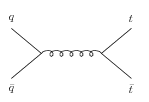
\includegraphics[width=0.2\textwidth]{theory/figures/toppairprod/qqbdiag}}
	\subfigure[]{\label{fig:ttprodgg}
  	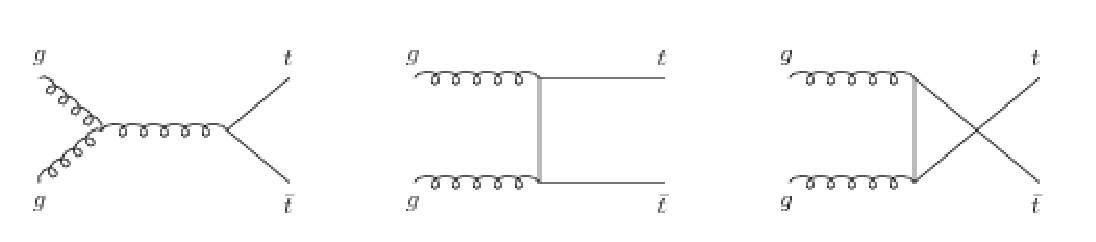
\includegraphics[width=0.65\textwidth]{theory/figures/toppairprod/ggdiag}}
	\caption{Pair production of top quarks from $q\bar{q}$ (a) 
          and $gg$ QCD interactions~\cite{Kidonakis:2011ca}. Pair
          production of heavy quarks is analogous.\label{fig:ttprod}}
\myskip
        \begin{fmffile}{fmfsingleprod}
\unitlength=1mm
  \begin{center}
\begin{fmfgraph*}(30,15)
  \fmfleft{i1,i2}
  \fmfright{o1,o2}
  \fmflabel{$q$}{i1}
  \fmflabel{$q'$}{i2}
  \fmflabel{$Q$}{o1}
  \fmflabel{$q_1$}{o2}
  \fmf{phantom}{o1,v1,i1}
  \fmf{phantom}{o2,v2,i2}
  \fmffreeze
  \fmf{plain}{o1,v1,i1}
  \fmf{plain}{o2,v2,i2}
  \fmf{photon,label=$V*$}{v1,v2}
\end{fmfgraph*}\hskip1cm
\begin{fmfgraph*}(30,15)
  \fmfleft{i1,i2}
  \fmfright{o1,o2}
  \fmflabel{$q$}{i1}
  \fmflabel{$q'$}{i2}
  \fmflabel{$Q$}{o1}
  \fmflabel{$q_1$}{o2}
  \fmf{phantom}{o1,v1,v2,i1}
  \fmf{phantom}{o2,v1,v2,i2}
%  \fmffreeze
  \fmf{plain}{o1,v1,o2}
  \fmf{plain}{i1,v2,i2}
  \fmf{photon,label=$V*$}{v1,v2}
\end{fmfgraph*}
  \end{center}
\end{fmffile}

        \caption{Examples of Feynman diagrams for single production of heavy qaurks $Q$.\label{fig:singleprod}}
\end{center}\end{figure}


\subsection{Decay}\label{sec:vlqdecay}

The electroweak interactions of the new heavy
quarks determine the possible decay channels of
the isosinglets and isodoublets.
In general, the allowed decay modes are:
\begin{align}
& T \to W^+ b \,, \quad T \to Zt \,,\quad T \to Ht;\label{eq:vltdec}\\
& B \to W^- t \,, \quad B \to Zb \,,\quad B \to Hb;\label{eq:vlbdec}\\
& X \to W^+ t;\\
& Y \to W^- b.
\end{align}
The flavor changing neutral currents entering in the
interactions of the $T$ and $B$ quarks come from the
breaxing of the GIM mechanism in the modified 
lagrangian~\cite{AguilarSaavedra:2009es}.

For the isospin singlets \Tlr\ and \Blr\ all the 
three decay modes of Equations~\ref{eq:vltdec} and~\ref{eq:vlbdec}
respectively are possible, while for isospin doublets different
options are present. Table~\ref{tab:vlqdec} summarizes the
allowed  decay modes for vector-like isosinglets and isodoublets.

In the case of the \TBlr\ doublet the two quarks
are almost degenerate in mass and the decays strongly depend
on the mixing factors of the extended CKM matrix $V_{Tb}$ and
$V_{tB}$. If $V_{Tb}\sim V_{tB}$ then the $T$ and $B$ quarks
have the same decays as the corresponding isosinglets but
different angular distributions since only the right-handed
component of \TBlr\ couples to the Standard Model quarks.
In the most natural case where $V_{Tb} \ll V_{tB}$ with the
Standard Model top quark, much heavier than the bottom quark,
mixes more strongly with the heavy quark, the $T\to W^+ b$
decay is suppressed as well as the $B\to Hb$ and 
$B \to Zb$, and this is the scenario considered in 
Table~\ref{tab:vlqdec}.

The $X$ and $T$ quarks of the \XTlr\ doublet are also
almost degenerate in mass and also in this case they
only couple to Standard Model quarks with the 
right-handed component. Here, however, charged currents
are not present in the first order lagrangian and hence the
decay $T\to W^+ b$ is not present, as reported in 
Table~\ref{tab:vlqdec}.
For the \BYlr\ doublet exactly the same arguments apply.


\begin{table}[htb]\centering
\begin{tabular}{|lc|lcc|}\toprule
\hskip2ex VLQ &  Decay & \hskip2ex VLQ & hyper- & Decay \\
\hskip1ex Singlets &  modes & \hskip1ex Doublets & charge & modes\\
& & & &\\%one empty line
$T(+2/3)$ & $W^+b,\, Ht,\, Zt$ &
\multirow{2}{*}{$\quad\bigg(\begin{array}{c}T \\ B\end{array}\bigg)$} & \multirow{2}{*}{$\dfrac{1}{6}$} & $ Ht,\, Zt$\\%$W^+b,\, Ht,\, Zt$\\
& & & & $ W^-t$\\%$ W^-t,\, Hb,\, Zb$\\
$B(-1/3)$ & $ W^-t,\, Hb,\, Zb$ & & & \\
& & \multirow{2}{*}{$\quad\bigg(\begin{array}{c}T \\ X\end{array}\bigg)$} & \multirow{2}{*}{$\dfrac{7}{6}$} & $Ht,\, Zt$\\
$X(+5/3)$ & $W^+t$ & & & $W^+t$\\
& & & &\\
$Y(-4/3)$ & $W^-b$ & \multirow{2}{*}{$\quad\bigg(\begin{array}{c}B \\ Y\end{array}\bigg)$} & \multirow{2}{*}{$-\dfrac{5}{6}$} & $Hb,\, Zb$\\
& & & & $W^-b$\\\bottomrule
\end{tabular}
	\caption{Allowed decay modes for vector-like isosinglets 
and isodoublets (the $L,R$ subscript is omitted).}\label{tab:vlqdec}
\end{table}


It is interesting to notice that for ``simple'' searches,
i.e. searches only aimed at revealing the presence of a new
heavy quark and not sensitive, e.g., to the particle charge
or angular distribution, a \Ylr\ will be indistinguishable from
a \BYlr\ or a chiral fourth generation $t'$. However it would be
possible to understand better the vector-like scenario by 
performing searches in the different decay channels in a 
model-independent way.

Decay ratios do not only depend on the model, but also
vary as a function of the heavy quark mass: Figure~\ref{fig:vlqbrs}
shows the decay branching ratios of the vector-like top and
bottom partners for isosinglets and isodoublets as a function
of the heavy quark mass, for a Higgs boson with mass $m_H=125~\gev$.

\begin{figure}
\centering
	\subfigure[]{\label{fig:vltbrs}
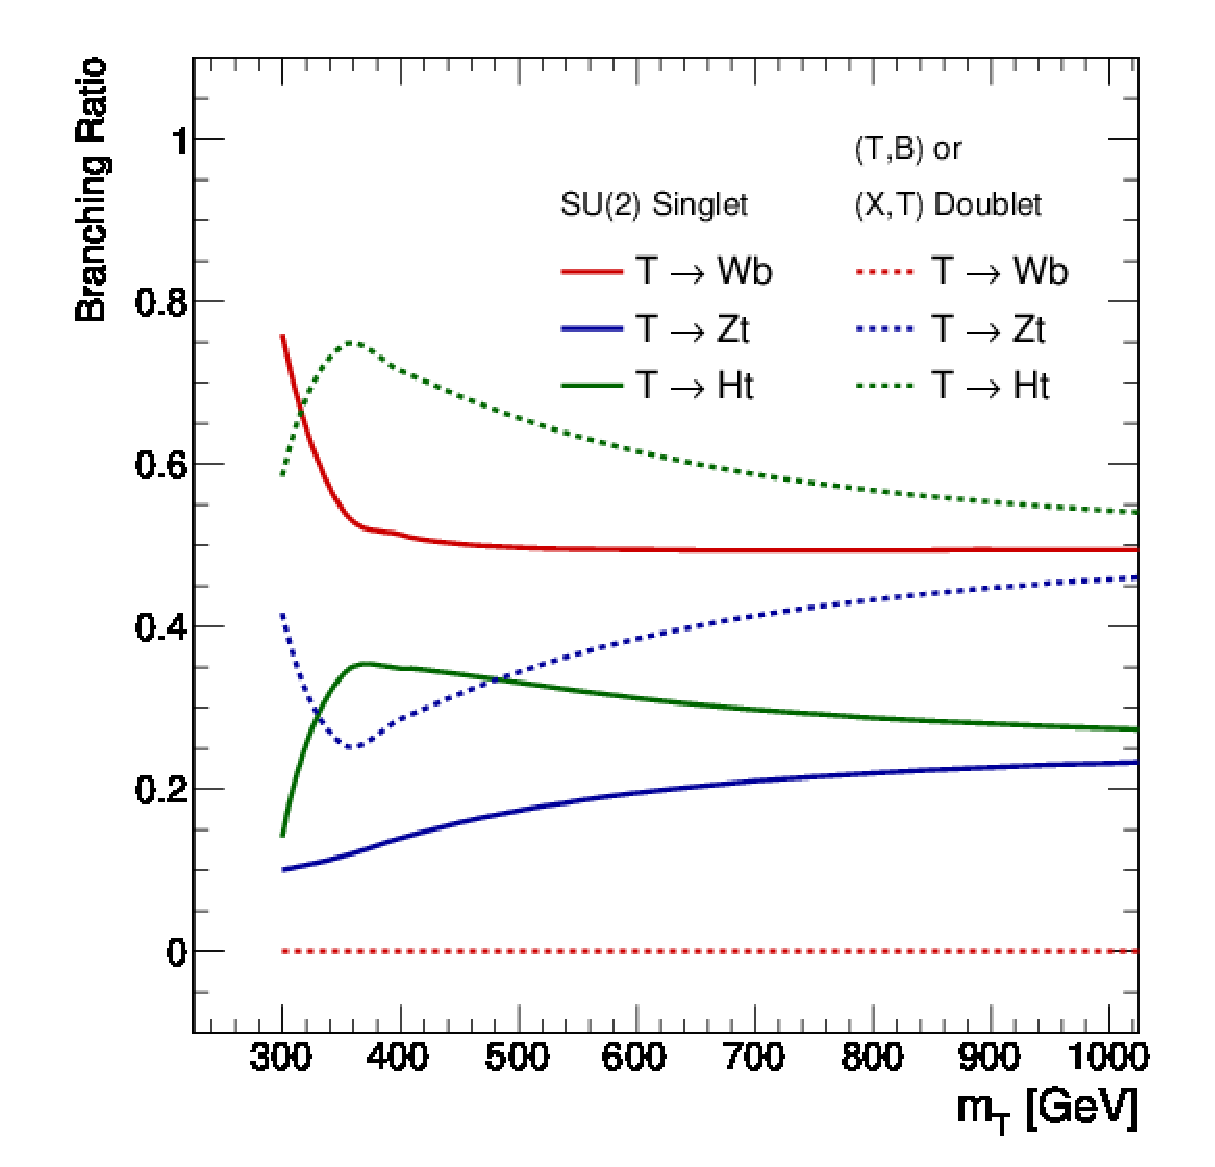
\includegraphics[width=.47\textwidth]{theory/figures/fig_02a}}
	\subfigure[]{\label{fig:vlbbrs}
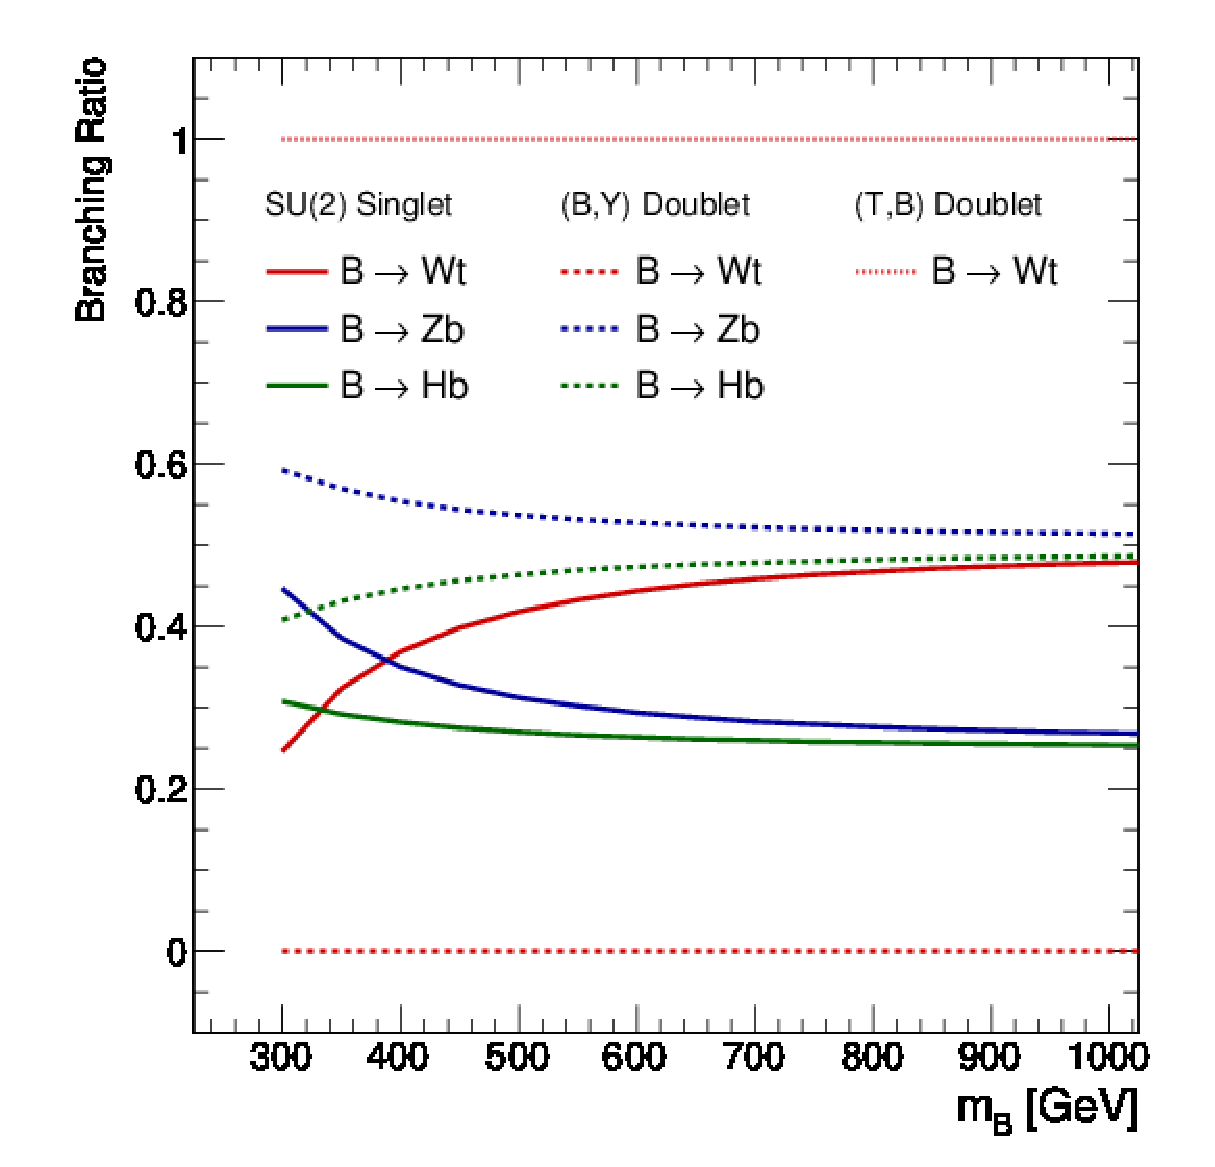
\includegraphics[width=.47\textwidth]{theory/figures/fig_02b}}
\caption{Branching ratio of vector-like top (a) and bottom (b) partners as a function of the heavy quark mass $m_T$ and $m_B$ respectively~\cite{ATLAS-CONF-2013-056} for isosinglets and isodoublets.}
\label{fig:vlqbrs}
\end{figure}

